\section{ContractNLI Dataset}\label{sec:dataset}

\subsection{Task Formulation}\label{sec:system-formulation}

Our task is, given a contract and a set of hypotheses (each being a sentence), to classify whether each hypothesis is \emph{entailed by}, \emph{contradicting to} or \emph{not mentioned by} (neutral to) the contract, and to identify \emph{evidence} for the decision as spans in the contract.
More formally, the task consists of:
\begin{description}
    \item[Natural language inference (NLI)] Document-level three-class classification (one of \textsc{Entailment}, \textsc{Contradiction} or \textsc{NotMentioned}).
    \item[Evidence identification] Multi-label binary classification over \emph{span}s, where a \emph{span} is a sentence or a list item within a sentence. This is only defined when NLI label is either \textsc{Entailment} or \textsc{Contradiction}.
\end{description}
% We chose such granularity for the span because presenting a clause would be too long to be useful and annotating by words would be too difficult for the annotators.
We argue that extracting whole sentences is more appropriate for ContractNLI because a lawyer can then check the evidence with comprehensible context around it, as oppose to the token-level span identification as in factoid question answering where users do not need to see the textual support for the answer.
Evidence spans therefore must be as concise as possible (need not be contiguous) while being self-contained, such that a reasonable user should be able to understand meaning just by reading the evidence spans (e.g., the second hypothesis in \cref{fig:task_overview} includes the first paragraph in order to clarify the clauses' subject).
We comprehensively identify evidence spans where they are redundant.

Unlike \cite{hendrycks_cuad_2021}, we target a single type of contracts.
This allows us to incorporate less frequent and more fine-grained hypotheses, as we can obtain a larger amount of such examples with the same number of annotated contracts.
While practioners will have to create a similar dataset to scale their system to another type of contracts, our work can be a model for how to generalize to other types of contracts because they would exhibit similar linguistic characteristics.
We chose non-disclosure agreements (NDAs) for our task, which are relatively easy to collect.

Because a lawyer would look for the same type of information in contracts of the same type, we fixed the hypotheses throughout all the contracts including the test dataset.
Given the closed set of hypotheses, this problem could also be addressed by building a text classifier for each hypothesis.
However, given the modest available data for a task requiring natural language understanding, we believe more power can be achieved by viewing this as an NLI problem.
Indeed, you can think of the NLI approach as building a multi-task text classifier with the hypothesis serving as a ``prompt'' to the model.
We will discuss whether introducing hypotheses is helpful to the model or not in \cref{sec:discussion-additional_experiments}.

\subsection{Data Collection}\label{sec:system-data}

In this section, we briefly discuss how we collected and annotated the dataset.
Since it posed many challenges that we cannot adequately describe within the page limit, we provide more details and caveats in \cref{sec:appendix-data-collection}.

\begin{figure*}[t]
    \centering
    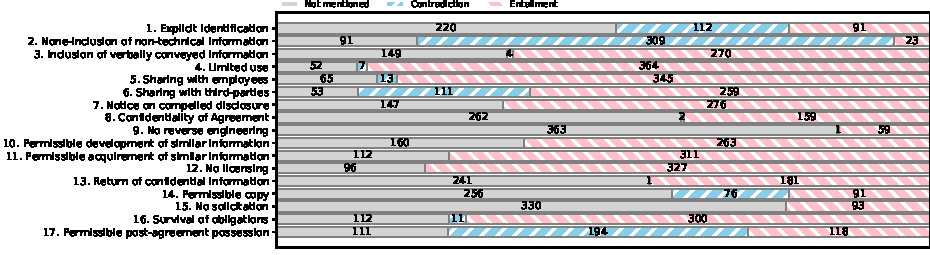
\includegraphics{fig/data-label_distribution}
    \caption{The NLI label distribution. Hypothesis names are used only for a human readability purpose. A full list of hypotheses can be found in \cref{tab:hypotheses}.}\label{fig:data-label_distribution}
\end{figure*}

\begin{table}[t]
    \centering
    \fontsize{8pt}{10pt}\selectfont
    \setlength{\tabcolsep}{4pt}
    \renewcommand{\arraystretch}{.6}
    \begin{tabular}{cccccc}\toprule
        Format & Source & Train & Development & Test & Total \\\midrule
        Plain Text & EDGAR & 83 & 12 & 24 & 119 \\
        HTML & EDGAR & 79 & 11 & 23 & 113\\
        PDF & Search engines & 261 & 38 & 76 & 375 \\\midrule
        \multicolumn{2}{c}{Total} & 423 & 61 & 123 & 607\\\bottomrule
    \end{tabular}
    \caption{Data split}\label{tab:data-split}
\end{table}

\begin{table}[t]
    \centering
    \fontsize{8pt}{10pt}\selectfont
    \setlength{\tabcolsep}{4pt}
    \renewcommand{\arraystretch}{.6}
    \begin{tabular}{ccccccc}\toprule
        & \multicolumn{3}{c}{Number per a document} & \multicolumn{3}{c}{Tokens per an instance} \\\cmidrule(lr){2-4}\cmidrule(lr){5-7}
        & Average & Min. & Max. & Average & Min. & Max.\\\midrule
        Paragraph & 43.7 & 9 & 248 & 52.8 & 1 & 1209 \\
        Span & 77.8 & 18 & 354 & 29.5 & 1 & 289 \\
        Token & 2,254.3 & 336 & 11,503 & --- & --- & --- \\\bottomrule
    \end{tabular}
    \caption{Basic statistics of the training dataset}\label{tab:data-tokens}
\end{table}


\begin{figure}[t]
    \centering
    \begin{subfigure}[b]{0.5\linewidth}
        \centering
        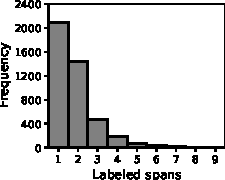
\includegraphics{fig/data-spans-num}
        \caption{As number of spans}
        \label{fig:data-spans-num}
    \end{subfigure}~
    \begin{subfigure}[b]{0.5\linewidth}
        \centering
        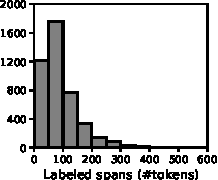
\includegraphics{fig/data-spans-len}
        \caption{As number of tokens}
        \label{fig:data-spans-len}
    \end{subfigure}
    \caption{Number of evidence spans in each document.}\label{fig:data-spans}
\end{figure}

We collected NDAs from Internet search engines and Electronic Data Gathering, Analysis, and Retrieval system (EDGAR).
We searched data with a simple regular expression and hand-picked valid contracts.

Since the collected documents came in various formats including PDFs, we used \cite{koreeda_capturing_2021} to extract plain text from the documents by removing line breaks, detecting paragraph boundaries and removing headers/footers.
In order to further ensure the quality of our data, we manually screened all the documents and corrected mistakes made by the tool.
We then used Stanza \cite{qi-etal-2020-stanza} to split each paragraph into sentences and further split each sentence at inline list items (e.g., at ``(a)'' or ``iv)'') using another regular expression.
Finally, we tokenized each sentence with Stanza and further split each token into subtokens using BERT's tokenizer \cite{devlin_bert_2019,wu_googles_2016}.

For hypotheses, we developed 17 hypotheses by comparing different NDAs.
We did not include hypotheses that would simply reason about presence of certain clauses (such as ``There exists an arbitration clause in the contract.'') because they are covered by previous studies \cite{leivaditi_benchmark_2020,hendrycks_cuad_2021}.

Finally, we annotated all the contracts based on the principles discussed in \cref{sec:system-formulation}.
Since we employ a fixed set of hypotheses unlike existing NLI datasets, we were able to utilize an example-oriented annotation guideline to improve annotation consistency.

\subsection{Data Statistics}\label{sec:dataset-statistics}

We annotated a total of 607 documents, which are split into training, development and testing data at a ratio of 70:10:20 stratified by their formats (\cref{tab:data-split}).
We show statistics of the documents in \cref{tab:data-tokens}.
A document on average has 77.8 spans to choose evidence spans from.
An average number of tokens per a document is 2,254.0, which is larger than maximum allowed context length of BERT (512 tokens).
Even though an NDA is relatively short for a contract, 86\% of documents exceed the maximum allowed context length of BERT.

The distribution of NLI labels is shown in \cref{fig:data-label_distribution}.
\textsc{Entailment} and \textsc{NotMentioned} occupy a significant ratio of the dataset, but around half of the hypotheses contain both \textsc{Entailment} and \textsc{Contradiction}.
The distribution of evidence spans is shown in \cref{fig:data-spans}.
The most of entailed/contradicting hypotheses have one or two evidence spans, but some have up to nine spans.

